\chapter{Théorème des résidus}
L'objectif de ce chapitre est d'étendre la formule de Cauchy à des domaines $n$-connexes, c'est-à-dire à considérer des applications holomorphes dans un domaine privé d'un nombre fini de points.
\section{Développement en série de Laurent}

\subsection{Série de Taylor d'une application holomorphe}

Nous avons vu que toute fonction $f$ holomorphe dans un domaine $\Omega$ de bord $\partial \Omega$, une courbe de Jordan régulière de classe $C^1$ par morceaux, et continue sur $\overline{\Omega}=\Omega \cup \partial \Omega$, y est indéfiniment dérivable. Montrons qu'une telle fonction est analytique dans $\Omega$.

Soit $z_0 \in \Omega$, le domaine étant ouvert, il existe $r>0$ tel que le disque ouvert $D(z_0 ;r) \subset \Omega$. La 
fonction $f$ étant holomorphe dans $D(z_0 ;r)$ et continue sur le bord du disque, nous pouvons appliquer la formule de Cauchy, qui donne pour tout $z \in D(z_0 ; r)$~:
\[f(z)=\frac{1}{2 \pi i}\int\limits_{\lvert z_0- u \rvert =r} \frac{f(u)}{u-z} \diff u.\]

%\begin{figure}
%\scalebox{.68}{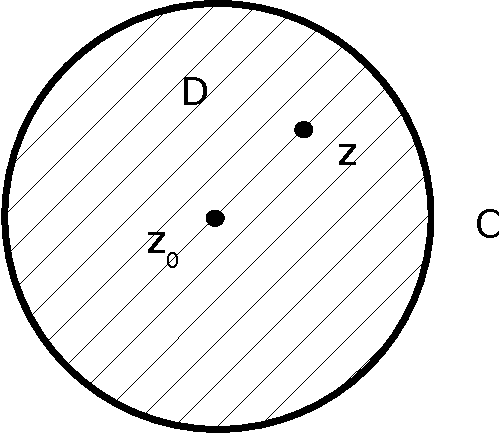
\includegraphics{images/taylor.pdf}}
%\caption{Domaine D}\label{Fi:Taylor}
%\end{figure}
Soit, en faisant intervenir le point $z_0$~:
\[
f(z) = \frac{1}{2\pi i}\int\limits_{\lvert z_0- u \rvert =r} \frac{f(u)}{(u-z_0)-(z-z_0)} \diff u =
\frac{1}{2\pi i}\int\limits_{\lvert z_0- u \rvert =r}
\frac{f(u)}{u-z_0}\frac{1}{1-\frac{z-z_0}{u-z_0}} \diff u.
\]
Pour un entier $N$ fixé, on a aussi~:
\[
\frac{1}{1-\frac{z-z_0}{u-z_0}} = \sum_{n=0}^N \left (\frac{z-z_0}{u-z_0}\right )^n + \left ( \frac{z-z_0}{u-z_0}
\right )^{N+1} \frac{(u-z_0)}{(u-z_0)-(z-z_0)}.
\]
L'application $f$ étant, par hypothèse, continue sur le cercle $\lvert z_0- u \rvert =r$ qui est compact, elle y est majorée en module par un réel $M>0$. Nous en déduisons la majoration de l'intégrale~:
\[
J=\int\limits_{\lvert z_0- u \rvert =r} \left ( \frac{z-z_0}{u-z_0}
\right )^{N+1} \frac{f(u)}{(u-z_0)-(z-z_0)} \diff u 
\]
par~:
\[\vert J \rvert \leq 2 \pi \left (\frac{\lvert z-z_0 \rvert}{r}
\right )^{N+1} \frac{Mr}{r-\lvert z-z_0 \rvert},
\]
car $\lvert z-z_0 \rvert <r$ (nous avons utilisé l'inégalité classique $\lvert z_1-z_2 \rvert \geq \bigl \lvert \lvert z_1\rvert-\lvert z_0 \rvert \bigr \rvert$). On en déduit la convergence de la série $f(z) = \sum_{n=0}^\infty a_n (z-z_0)^n$, avec 
\[a_n= \frac{1}{2 \pi i}\int\limits_{\lvert z_0- u \rvert =r} \frac{f(u)}{(u-z_0)^{n+1}}  \diff u. \]
Par application de la formule de Cauchy, nous obtenons que
\[a_n= \frac{f^{(n)}(z_0)}{n!}\]
d'où un développement en série de Taylor de $f$ en tout
point $z \in D(z_0;r)$~:
\[
f(z)= \sum_{n=0}^\infty \frac{f^{(n)}(z_0)}{n!} (z-z_0)^n.\]

Il est clair que ce développement en série de Taylor de $f$ est
unique. On en déduit également que toute fonction holomorphe dans un domaine $\Omega$ de bord convenable, et continue sur $\overline{\Omega}$ est analytique dans $\Omega$.

\subsection{Série de Laurent d'une application holomorphe dans une couronne}

La série de Taylor est adaptée pour représenter les fonctions analytiques dans des disques. Lorsque la fonction est holomorphe le voisinage d'un point $z_0$, excepté ce point, il est nécessaire de considérer des domaines annulaires de la forme $r< \lvert z-z_0 \rvert <R$, avec $r>0$ et $R \leq \infty$. 

\begin{figure}[H]
\begin{center}
\shorthandoff{!}\shorthandoff{:}
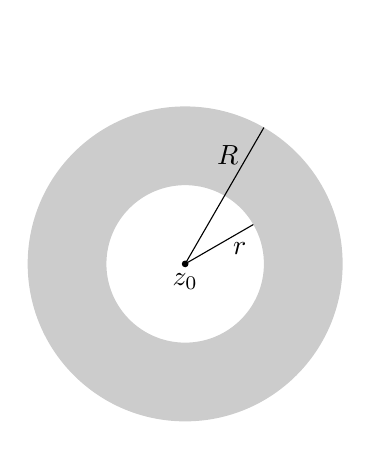
\begin{tikzpicture}
\clip(-2,-2) rectangle (2,3);
%\begin{scope}[xshift=7 cm]
% \tikzstyle{point}=[circle,thick,draw=black,fill=black,inner sep=0pt,minimum width=4pt,minimum height=4pt]
%    \fill[color=gray!40] (-2,0) -- (-1,0.5) -- (0,2) -- (1,0.5) -- (2,0) -- (1,-0.5) -- (0,-2) -- (-1,-0.5) -- cycle;
%    \node (a)[point,label=$z_0$] at (0,0) {};
%\end{scope}
\fill[color=gray!40,even odd rule] (0,0) circle(1) circle(2);
\draw [fill=black] (0,0) circle (1pt);
 \draw (0,0) node[below]{$z_0$} ;
 \draw (0.,0.)-- ++(60:2);
 \draw (0.,0.)-- ++(30:1);
 \draw (0.,0.)++(60:1.6) node[left] {$R$};
  \draw (0.,0.)++(30:0.8) node[below] {$r$};
\end{tikzpicture}
\shorthandon{!}\shorthandoff{:}
%\caption{}
\end{center}
\end{figure}


L'anneau ainsi considéré a pour contour la réunion des deux cercles centrés en $z_0$ et de rayons respectifs $r$ et $R$. Le cercle $\lvert z-z_0\rvert =R$ sera orienté positivement en sens
trigonométrique, le cercle $\lvert z-z_0\rvert =r$ sera orienté en sens inverse
trigonométrique (le bord reçoit ainsi son orientation canonique). Par
application de la formule de Cauchy et en tenant compte des orientations, on obtient pour tout $z$ dans la couronne~:
\[
f(z) = \frac{1}{2 \pi i} \int\limits_{\lvert u-z_0\rvert =R} \frac{f(u)}{u-z} \diff u - \frac{1}{2
\pi i} \int\limits_{\lvert u-z_0\rvert =r} \frac{f(u)}{u-z} \diff u
.\]
La première intégrale de la partie droite se développe de la même façon que
précédemment et l'on obtient une série de la forme $\sum_{n=0}^\infty a_n(z-z_0)^n$, avec~:
\[
a_n = \frac{1}{2\pi i} \int\limits_{\lvert u-z_0\rvert =R}  \frac{f(u)}{(u-z_0)^{n+1}} \diff u
\]
\begin{rem}
Bien prendre garde à ne pas écrire $a_n=f^{(n)}(z_0)/n!$ car $f$ n'est
pas supposée holomorphe au voisinage de $z_0$.
\end{rem}
Pour la seconde intégrale, on utilisera l'expression suivante~:
\[
\frac{1}{z-u} = \frac{1}{z-z_0}\frac{1}{1-
\frac{u-z_0}{z-z_0}} =\frac{1}{z-z_0} + \frac{(u-z_0)}{(z-z_0)^2} + \cdots + \frac{(u-z_0)^{n-1}}{(z-z_0)^n} + \cdots,
\]
série qui converge uniformément puisque $\vert (u-z_0)/(z-z_0)\rvert <1$. En procédant de façon analogue à l'expression de la première intégrale, on obtient l'expression suivante pour le deuxième terme de gauche~:
\[
- \frac{1}{2 \pi i} 
\int\limits_{\lvert u-z_0\rvert =r} \frac{f(u)}{u-z} \diff u = \sum_{n \geq 1} b_n(z-z_0)^{-n}\]
avec
\[b_n = \frac{1}{2\pi i} \int\limits_{\lvert u-z_0\rvert =r} (u-z_0)^{n-1}f(u) \diff u, \quad n=1,2,\cdots\]
En réunissant les deux séries, nous obtenons le développement suivant~:
\begin{align*}
f(z) &= \sum_{n=-\infty}^\infty c_n (z-z_0)^n,
\intertext{avec}
c_n& = \frac{1}{2 \pi i}\int_\gamma \frac{f(u)}{(u-z_0)^{n+1}} \diff u, \quad n=0, \pm 1, \pm 2, \cdots,
\end{align*}
où $\gamma = \lvert z-z_0\rvert = \rho$, $r< \rho <R$ est un lacet simple homotope aux deux bords de l'anneau, d'orientation positive pour $n \geq 0$, négative pour $n < 0.$

\begin{fdefn}
Le développement en série ainsi obtenu :
\[ f(z)  = \sum_{n=-\infty}^\infty c_n (z-z_0)^n \] est appelé \textbf{développement de Laurent} de $f$ dans la couronne de centre $z_0$. \\
La série pour $n \geq 0$ est appelée \textbf{partie régulière} et la série pour $n \leq -1$ est appelée \textbf{partie principale}. \\ 
Ce développement est valable en tout point de la couronne d'analyticité.
\end{fdefn}

Tout comme le développement en série de Taylor, le développement en série de Laurent est unique, ses coefficients s'exprimant par une intégrale de chemin. 
 \begin{exercice}
 Déterminer le développement en série de Laurent en $0$ et en $i$ de l'application:
 \[
 z \mapsto \frac{e^z}{z^2+1}
 \]
 \end{exercice}

\section{Points singuliers}

Un point $a \in \C$ est appelé \textbf{point singulier isolé} d'une fonction $f$, s'il existe un voisinage ouvert $0< \lvert z-a \rvert <R$ de ce point dans lequel $f$ est holomorphe. Par exemple, le point $z=0$ est un point singulier non isolé pour la fonction $\log z$, qui n'est définie dans aucun disque centré en $0$ et privé de ce point.

On distingue trois types de points singuliers isolés~:
\begin{enumerate}
\item $a$ est un point singulier \textbf{artificiel} si $\lim_{z \to a} f(z)$ existe et est finie;
\item $a$ est un \textbf{pôle} si $\lim_{z \to a} \lvert f(z) \rvert = + \infty$;
\item $a$ est un point singulier \textbf{essentiel} si $\lim_{z \to a} f(z)$ n'existe pas. 
\end{enumerate}

Si $a$ est un point singulier isolé d'une fonction $f$, il existe alors un développement en série de Laurent dans le voisinage $0< \lvert z-a \rvert <R$, dont la nature varie en fonction de la catégorie du point singulier.

\begin{fprop}\label{prop:riemann}Pour qu'un point $a$ soit un point singulier artificiel d'une fonction $f$, il faut et il suffit que le développement en série de Laurent de $f$ au voisinage de $a$ ne contienne pas de partie principale.
\end{fprop}
\begin{proof}
Si la série de Laurent de $f$ au voisinage de $a$ ne contient pas de partie principale, alors $a$ est un point singulier artificiel ; la valeur de $f$ en ce point est $c_0$. Réciproquement, si $a$ est artificiel, alors $\lim_{z \to a} f(z)$ existe et est finie, donc $f$ est bornée en module dans un voisinage de $a$ par une constante $M$. Les inégalités de Cauchy montrent que $\lvert c_n \rvert \leq M \rho^{-n}$ pour tout $\rho>0$. Pour $n<0$, cette borne tend vers $0$ lorsque $\rho \to 0$, nous en déduisons que $c_n=0$, pour tout $n<0$. 
\end{proof}

\begin{rem} Nous avons en fait montré que si $f$ est bornée dans un voisinage d'un point isolé $a$, alors $a$ est un point singulier artificiel. 
\end{rem}

\begin{fprop} Pour qu'un point $a$ soit un pôle d'une fonction $f$, il faut et il suffit que la partie principale du développement en série de Laurent de $f$ au voisinage de $a$ ne contienne qu'un nombre fini de termes, c'est à dire qu'il existe $N>0$ tel qu'au voisinage de $a$
\[ f(z)=\frac{c_{-N}}{(z-a)^N} + \cdots + \frac{c_{-1}}{(z-a)} + \sum_{n=0}^\infty c_n(z-a)^n.\]
L'entier $N$ est appelé l'\textbf{ordre} du pôle $a$, il est défini par $c_{-N} \neq 0$ et $c_{k} = 0$ pour tout $k <-N$.  
\end{fprop}

\begin{proof}
Si $a$ est un pôle de $f$, alors la fonction $1/f(z)$ tend vers zéro lorsque $z \to a$ ; donc $a$ est un zéro isolé de la fonction $1/f$. Soit $N$ l'ordre du zéro de $1/f$, on en déduit que $f(z)=g(z)/(z-a)^N$ avec $g$ holomorphe en $a$ et $g(a) \neq 0$. La fonction $g$ est développable en série de Taylor au voisinage de $a$
\begin{align*}
g(z)&=c_{-N} + c_{-N+1} (z-a)  + \cdots + c_0(z-a)^N + c_1(z-a)^{N+1} + \cdots,\\
\intertext{d'où}
f(z)&= \frac{c_{-N}}{(z-a)^N} + \frac{c_{-N+1}}{(z-a)^{N-1}} + \cdots + c_0 + c_1 (z-a) + \cdots.
\end{align*}
\end{proof}

Nous en déduisons alors la proposition suivante~:
\begin{prop}
Un point $a$ est un point singulier essentiel d'une fonction $f$, si et seulement si la partie principale de son développement en série de Laurent au voisinage de $a$ contient une infinité de termes.
\end{prop}

Le comportement d'une fonction au voisinage d'un point singulier essentiel est décrit par le théorème suivant
\begin{theorem}
Si $a$ est un point singulier essentiel d'une fonction $f$ holomorphe dans $\Omega \setminus\{a\}$, alors si $r>0$ et et $D(a;r) \subset \Omega$, l'image $f(D(a;r))$ est dense dans le plan complexe. Cela signifie que pour tout nombre complexe $\omega_0$, il existe une suite $z_n  \to_a$ telle que $f(z_n) \to \omega_0$.
\end{theorem}
\begin{proof}
Supposons la proposition fausse, donc qu'il existe un complexe $\omega_0$ qui ne soit pas limite de $f(z_n)$ pour $z_n \to a$. Il existe donc un $\epsilon>0$ petit tel que $\lvert f(z)-\omega_0 \rvert > \epsilon$ pour tout $z$ proche de $a$. Alors la fonction $h(z)=1/(f(z)-\omega)$ est bornée dans un voisinage de $a$. D'après la remarque faisant suite à la proposition~\ref{prop:riemann}, $a$ est un point singulier artificiel. Ainsi, $h(z)=(z-a)^N g(z)$ pour un $N \geq 0$ et une fonction holomorphe $g$ telle que $g(a) \neq 0$. Par conséquent $f(z)-a=(z-a)^{-N}(1/g(z))$ où $1/g(z)$ est holomorphe en $a$. Si $N=0$, alors $f(z)$ s'étend analytiquement en $a$, tandis que si $N>0$, $f(z)$ admet un pôle d'ordre $N$ en $a$.
\end{proof}

\begin{exem}
\begin{MYenumerate}
\item Les fonctions $\sin z/z$, $(1-e^z)/z$ et $(1-\cos z)/z$ ont l'origine pour point singulier artificiel.
\item La fonction $f(z)=1/(\exp(z^2) +1)$ possède des pôles aux points $z_n = \pm \sqrt{(2k+1) \pi i}$, $k=0, \pm 1, \pm 2, \cdots,$. Ils sont tous du premier ordre, puisque la fonction $1/f(z)$ a ces points pour zéros d'ordre $1$.
\item Les fonctions $e^{1/z}$, $\sin(1/z)$, $\cos(1/z)$ ont l'origine pour point singulier essentiel. Notons que $f(z)=e^{1/z}$ :
\begin{itemize}
\item si $z_n=1/n$, alors $f(z_n) \to \infty$ ;
\item si $z_n=-1/n$, alors $f(z_n) \to 0$ ;
\item et enfin, soit $\omega \neq 0$ fini et soit $z_n=1/(\log \omega + 2 n \pi i)$ (avec la détermination principale du logarithme), alors $f(z_n) \to \omega$.
\end{itemize}
Ceci illustre la propriété d'un point singulier essentiel ;
\item $f(z)=1/(\exp(1/z^2) + 1)$ a l'origine comme point singulier non isolé, car ses pôles $z_n = \pm 1/\sqrt{(2k+1) \pi i}$ ont l'origine comme point adhérent.
\end{MYenumerate}
\end{exem}

Une fonction $f(z)$ est dite \textbf{méromorphe} dans un domaine du plan complexe si $f$ y est holomorphe sauf en des points singuliers isolés, chacun d'eux étant un pôle. Plus généralement, les fonctions méromorphes sont localement de la forme $g(z)/h(z)$ avec $g,h$ holomorphes.


\section{Théorème des résidus}
Les résultats de la section précédente permettent de développer une application
$f$ au voisinage d'un point singulier isolé $a$. On notera le lien existant
entre $c_{-1}$ et l'intégrale de l'application sur le cercle intérieur d'une couronne
entourant le point singulier. Ce coefficient, en raison de son importance,
a reçu un nom particulier~: c'est le \textbf{résidu} de $f$ en $a$, noté $\text{Res}(f;a)$. Nous avons la relation importante suivante~:
\[\text{Res}(f;a) = \frac{1}{2 \pi i} \int_\gamma f(z) \diff z,\]
où $\gamma$ est le cercle $\lvert z-a\rvert =\rho$ avec $\rho$ suffisamment petit. Il est possible de remplacer $\gamma$ par tout lacet simple homotope dans le domaine considéré. Si, au lieu de prendre le cercle on considère un lacet entourant plusieurs fois $a$, il faut introduire l'indice du chemin par rapport à $a$.  


Énonçons maintenant le théorème des résidus, un théorème fondamental et à la base du calcul des intégrales de chemin.  

%\begin{fthm}
%Soit $f$ une fonction méromorphe dans un domaine borné et simplement connexe $\Omega$ du plan complexe. Soit $A$ l'ensemble des points de $\Omega$ en lesquels $f$ a un pôle. Soit $\gamma$ un lacet dans $\Omega \setminus A$, alors
%\begin{equation}\label{eq:residu1}
%\frac{1}{2 \pi i} \int_\gamma f(z)\diff z = \sum_{a \in A} \text{Res}(f;a) I(\gamma ; a).
%\end{equation}
%\end{fthm}
%
%\begin{proof}
%Comme $\Omega$ est borné, et comme les points de $A$ sont isolés, on en déduit que $A$ est un ensemble fini et la somme dans~(\ref{eq:residu1}), formellement infinie, est en réalité finie. Soient $a_1, \cdots, a_n$ les points de $A$ et $h_1,\cdots, h_n$ les parties principales de $f$ en $a_1,\cdots, a_n$, posons $g=f-(h_1 + \cdots h_n)$. Alors $g$ a des singularités artificielles en $a_1,\cdots, a_n$ et donc $\int_\gamma g = 0$. Comme le seul pôle de $h_k$ est $a_k$, il s'ensuit que
%\[\frac{1}{2 \pi i} \int_\gamma f(z)\diff z = \sum_{k =1}^n \text{Res}(h_k;a_k) I(\gamma ; a_k),\]
%et comme $f$ et $h_k$ ont même résidus en $a_k$, on obtient~(\ref{eq:residu1}).
%\end{proof}
%
%%\begin{fthm}
%%Soit $\Omega$ un ouvert simplement connexe et soit 
%%$\gamma$ un lacet de $\Omega$ . Soit $f$ une application holomorphe dans 
%%$\Omega-\{z_1, \dots z_n\}$ où les $z_i,i=1\dots n$ sont distincts deux à deux.
%%O~:
%%\[
%%\int_{\gamma} f(z) dz = i 2 \pi \sum_{j=1}^n Res(f;z_i) I(\gamma;z_k)
%%\]
%%\end{fthm}
%%
%%\begin{proof}
%%Il existe pour chaque $z_j$ une
%%couronne ouverte $\mathcal{C}_j$ de centre $z_j$ ne contenant aucun autre point
%%singulier. Le développement en série de Laurent sur chacune de ces couronnes
%%montre que~:
%%\[
%%Res_{z_j}f = \frac{1}{i 2 \pi} \int_{c_j} f(z) dz
%%\]
%%avec $c_j$ cercle intérieur de $\mathcal{C}_j$, orienté en sens
%%trigonométrique. L'application $f$ étant holomorphe dans $\Omega - \cup_{j=1}^n
%%D_j$ avec $D_j$ disque ouvert de centre $z_j$ et de bord $c_j$, on a~:
%%\[
%%\int_{\gamma} f(z) dz - \sum_{j=1}^n \int_{c_j} f(z)dz =0
%%\]
%%et le résultat s'en déduit.
%%\end{proof}
%%\begin{rem}
%%Le calcul pratique des résidus d'une application $f$ peut s'obtenir par
%%développement en série de Laurent. Dans le cas d'un pôle simple en $z_0$, on
%%retiendra que si $f(z)=p(z)/q(z)$, alors~:
%%\[
%%Res_{z_0}f = \frac{p(z_0)}{q^\prime(z_0)}
%%\]
%%Si on a affaire a un pôle d'ordre $p$, on utilisera la formule~:
%%\[
%%Res_{z_0}f = \lim_{z \to z_0} \frac{1}{(p-1)!}
%%\frac{d^{p-1}}{dz^{p-1}}[(z-z_0)f(z)]
%%\]
%%\end{rem}
%
%Il existe une forme du théorème des résidus plus utile au calcul d'une intégrale complexe.

\begin{fthm}
Soit $\Omega$ un domaine simplement connexe. Soit $f$ holomorphe dans $\Omega$, sauf en un nombre fini de points singuliers $z_1, \cdots, z_m$. Alors, pour tout lacet $\gamma$ ne passant par aucun des $z_i, i = 1 \dots m$:
\begin{equation}\label{eq:residu1}
\int_{\gamma} f(z) \diff z = 2 \pi i \sum_{j=1}^m I(\gamma;z_i) \text{ Res}(f ; z_i).
\end{equation}
\end{fthm}

\begin{proof}
Soit $\Omega_\epsilon$ le domaine obtenu à partir de $\Omega$ en retirant des petits disques $D_j$ centrés en $z_j$ et de rayon $\epsilon$ tels que $\gamma$ reste un lacet dans $\Omega_\epsilon$.
\begin{figure}[H]
\begin{center}
\shorthandoff{!}\shorthandoff{:}
\begin{tikzpicture}[line cap=round,line join=round,>=triangle 45,x=1.0cm,y=1.0cm, scale=0.7]
\tikzset{
  % style to apply some styles to each segment of a path
  on each segment/.style={
    decorate,
    decoration={
      show path construction,
      moveto code={},
      lineto code={
        \path [#1]
        (\tikzinputsegmentfirst) -- (\tikzinputsegmentlast);
      },
      curveto code={
        \path [#1] (\tikzinputsegmentfirst)
        .. controls
        (\tikzinputsegmentsupporta) and (\tikzinputsegmentsupportb)
        ..
        (\tikzinputsegmentlast);
      },
      closepath code={
        \path [#1]
        (\tikzinputsegmentfirst) -- (\tikzinputsegmentlast);
      },
    },
  },
  % style to add an arrow in the middle of a path
  mid arrow/.style={postaction={decorate,decoration={
        markings,
        mark=at position .5 with {\arrow[#1]{stealth}}
      }}},
}
\clip(0,-5) rectangle (29.78,4);
\draw [rotate around={0.:(4.5,0.)},line width=1.2pt,postaction={on each segment={mid arrow=black}}, fill=gray!40] (4.5,0.) ellipse (4.144842282494378cm and 2.2202967249341268cm);
\draw [rotate around={61.23235066115617:(2.04,-0.03)},line width=1.2pt, fill=white,decoration={markings, mark=at position 0.3 with {\arrow{stealth reversed}}},
        postaction={decorate}] (2.04,-0.03) ellipse (0.8324871889049981cm and 0.5954283497541448cm);
\draw [rotate around={-52.35237935989236:(6.8,0.02)},line width=1.2pt,fill=white,decoration={markings, mark=at position 0.3 with {\arrow{stealth reversed}}},
        postaction={decorate}] (6.8,0.02) ellipse (1.0041314413829652cm and 0.47610918030830296cm);
\draw [rotate around={0.:(17.63,0.)},line width=1.2pt,postaction={on each segment={mid arrow=black}},fill=gray!40] (17.63,0.) ellipse (4.201522428883097cm and 2.1156301000901205cm);
\draw [rotate around={61.23235066115615:(14.9,-0.23)},line width=1.2pt,fill=white,decoration={markings, mark=at position 0.3 with {\arrow{stealth reversed}}},
        postaction={decorate}] (14.9,-0.23) ellipse (0.8324871889049802cm and 0.595428349754132cm);
\draw [rotate around={-52.352379359892396:(19.66,-0.18)},line width=1.2pt,fill=white,decoration={markings, mark=at position 0.3 with {\arrow{stealth reversed}}},
        postaction={decorate}] (19.66,-0.18) ellipse (1.0041314413828102cm and 0.4761091803082292cm);

\draw [line width=1.2pt, fill=white,decoration={markings, mark=at position 0.3 with {\arrow{stealth reversed}}},
        postaction={decorate}] (16.16,-1.36) circle (0.42755116652863884cm);
\draw [line width=1.2pt, fill=white,,decoration={markings, mark=at position 0.3 with {\arrow{stealth reversed}}},
        postaction={decorate}] (17.3,-0.78) circle (0.45122056690713946cm);
\draw [line width=1.2pt, fill=white,,decoration={markings, mark=at position 0.3 with {\arrow{stealth reversed}}},
        postaction={decorate}] (18.14,0.48) circle (0.4103656905736646cm);
\begin{scriptsize}
\draw [fill=black] (3.3,-1.16) circle (2.0pt);
\draw[color=black] (3.61,-0.78) node {\normalsize $z_1$};
\draw [fill=black] (4.44,-0.58) circle (2.0pt);
\draw[color=black] (4.75,-0.2) node {\normalsize $z_2$};
\draw [fill=black] (5.28,0.68) circle (2.0pt);
\draw[color=black] (5.59,1.06) node {\normalsize $z_3$};
\draw [fill=black] (16.16,-1.36) circle (2.0pt);
\draw [fill=black] (17.3,-0.78) circle (2.0pt);
\draw [fill=black] (18.14,0.48) circle (2.0pt);
\end{scriptsize}
\end{tikzpicture}
\shorthandon{!}\shorthandoff{:}
\end{center}
\end{figure}

La formule de calcul du résidu en $z_j$ donne 
\[\int_{\partial D_j} f(z) \diff z = 2 \pi i \text{ Res}(f ; z_j).\]
Par ailleurs, le théorème de Cauchy et l'invariance par homotopie donne
\[0=\int_{\partial \Omega_\epsilon} f(z) \diff z = \int_{\gamma} f(z)  \diff z - \sum_{j=1}^m I(\gamma;z_i) \int_{\partial D_j} f(z) \diff z.\]
Nous obtenons~(\ref{eq:residu1}) en combinant les deux identités.
\end{proof}

Le théorème des résidus permet de calculer une quantité \og globale\fg{}, qu'est une intégrale de chemin, à partir de quantités locales : les résidus. Par exemple, pour calculer l'intégrale généralisée $\int_{-\infty}^\infty f(x) \diff x$, où $f$ est la restriction à l'axe réel d'une fonction (notée aussi $f$) holomorphe dans un domaine $\Omega$ contenant le demi-plan $\text{Im} z \geq 0$ sauf en un certain nombres de pôles. On considère un contour de la forme ci-dessous, où nous avons supposé l'absence de pôles sur l'axe réel.

\begin{figure}[H]
\begin{center}
\shorthandoff{!}\shorthandoff{:}
\begin{tikzpicture}[domain=0:4]

\tikzset{
  % style to apply some styles to each segment of a path
  on each segment/.style={
    decorate,
    decoration={
      show path construction,
      moveto code={},
      lineto code={
        \path [#1]
        (\tikzinputsegmentfirst) -- (\tikzinputsegmentlast);
      },
      curveto code={
        \path [#1] (\tikzinputsegmentfirst)
        .. controls
        (\tikzinputsegmentsupporta) and (\tikzinputsegmentsupportb)
        ..
        (\tikzinputsegmentlast);
      },
      closepath code={
        \path [#1]
        (\tikzinputsegmentfirst) -- (\tikzinputsegmentlast);
      },
    },
  },
  % style to add an arrow in the middle of a path
  mid arrow/.style={postaction={decorate,decoration={
        markings,
        mark=at position .5 with {\arrow[#1]{stealth}}
      }}},
}

\draw [<->, very thick] (0,4) node (yaxis) [above] {$y$}
    |- (-4,0) node (zaxis) [left] {}
    |- (4,0) node (xaxis) [right] {$x$}
    ;
   \path [color=blue,draw=black, ultra thick, postaction={on each segment={mid arrow=black}}] (3,0) arc (0:180:3cm)
    (-3,0) -> (3,0) ;
    \draw (-3,0) node[below]{$-R$};
    \draw (3,0) node[below]{\normalsize $R$};
%    (-1,0) arc (180:0:1cm) % changed starting point and swapped arc bounding angles
%    (-3,0) -> (-1,0) ; % swapped coordinates here
\draw [fill=black] (-2,0.3) circle (2.0pt);
\draw[color=black] (-1.9,0.5) node {\normalsize $a_1$};
\draw [fill=black] (1,0.5) circle (2.0pt);
\draw[color=black] (1.1,0.7) node {\normalsize $a_2$};
\draw [fill=black] (2,1.5) circle (2.0pt);
\draw[color=black] (2.1,1.7) node {\normalsize $a_3$};
\draw[color=black] (1,3.2) node {\normalsize $\gamma_2$};
\draw[color=black] (1, -0.5) node {\normalsize $\gamma_1$};
\end{tikzpicture}

\shorthandon{!}\shorthandoff{:}


\end{center}
\end{figure}

On applique le théorème des résidus au domaine délimité par le lacet $\gamma=\gamma_1 + \gamma_2$, ce qui conduit à l'identité
\[\int_{-R}^R f(x) \diff x + \int_{\gamma_2} f(z) \diff z = 2 \pi i \sum_{k=1}^n \text{Res}(f;a_k).\]
Si en outre, il est possible de prouver que $\lim_{R \to \infty} \int_{\gamma_2} f(z) \diff z =0$ (par application du lemme de Jordan par exemple), on obtient alors la valeur de l'intégrale généralisée
\[\int_{-\infty}^\infty f(x) \diff x = \lim_{R \to \infty}  \int_{-R}^R f(x) \diff x = 2 \pi i \sum \text{Res}(f;a),\]
où la somme porte sur tous les pôles inclus dans le demi-plan supérieur.

Si l'axe réel contient un pôle (par ex. l'origine), il faudra l'exclure (ou l'inclure) dans le domaine en considérant un contour de la forme ci-dessous

\begin{figure}[H]
\begin{center}
\shorthandoff{!}\shorthandoff{:}
\begin{tikzpicture}[domain=0:4]

\tikzset{
  % style to apply some styles to each segment of a path
  on each segment/.style={
    decorate,
    decoration={
      show path construction,
      moveto code={},
      lineto code={
        \path [#1]
        (\tikzinputsegmentfirst) -- (\tikzinputsegmentlast);
      },
      curveto code={
        \path [#1] (\tikzinputsegmentfirst)
        .. controls
        (\tikzinputsegmentsupporta) and (\tikzinputsegmentsupportb)
        ..
        (\tikzinputsegmentlast);
      },
      closepath code={
        \path [#1]
        (\tikzinputsegmentfirst) -- (\tikzinputsegmentlast);
      },
    },
  },
  % style to add an arrow in the middle of a path
  mid arrow/.style={postaction={decorate,decoration={
        markings,
        mark=at position .5 with {\arrow[#1]{stealth}}
      }}},
}


\draw [<->,  thick] (0,4) node (yaxis) [above] {$y$}
    |- (-4,0) node (zaxis) [left] {}
    |- (4,0) node (xaxis) [right] {$x$}
    ;
   \path [draw=blue, ultra thick, postaction={on each segment={mid arrow=black}}] (3,0) arc (0:180:3cm)
    (1,0) -> (3,0)
    (-1,0) arc (180:0:1cm) % changed starting point and swapped arc bounding angles
    (-3,0) -> (-1,0) ; % swapped coordinates here

    \draw (-3,0) node[below]{$-R$};
    \draw (3,0) node[below]{\normalsize $R$};
   \draw (-1,0) node[below]{\normalsize $-\epsilon$};
    \draw (1,0) node[below]{\normalsize $\epsilon$};

\end{tikzpicture}

\shorthandon{!}\shorthandoff{:}


\end{center}
\end{figure}


\begin{exercice}
\label{ex:int_gen}
Calculer les intégrales généralisées suivantes~:

\begin{align*}
I_1 & = \int_0^{+\infty} \frac{x^2 \cos(ax)}{1+x^4} \diff x , \quad a \in
\mathbb{R}\\
I_2 & = \int_0^{+\infty} \frac{ \sin x}{x}\diff x
\end{align*}

\end{exercice}
%\section{Calcul numérique}
%Les développements en série de Laurent permettent souvent d'approcher numériquement une fonction inconnue ou très difficile à calculer par une fraction rationnelle complexe. Le site:
%\url{http://dlmf.nist.gov/} recense de très nombreuses fonctions, avec des méthodes permettant de les calculer. On y trouvera des expressions sous formes de fractions continues, dont la troncature à un ordre fini donne une fraction rationnelle. Dans certains cas, une approximation rationnelle est beaucoup plus efficace qu'un développement en série de Taylor. 
%
%On supposera dans la suite que la fonction $f$ que l'on souhaite approcher est connue de façon expérimentale, sous la forme d'un échantillon de couples de complexes $(z_i,w_i), i=0 \dots N-1$ avec $w_i = f\left(z_i\right)$. On recherchera une fraction rationnelle:
%\[
%\widetilde{f} \colon z \mapsto \frac{\sum_{k=0}^P a_k z^k}{\sum_{j=0}^Q b_j z^j}
%\]
%qui minimise l'erreur de calcul:
%\[
%\sum_{i=0}^{N-1} \left|w_i - \widetilde{f}(z_i)\right|^2
%\] 
%Sous cette forme, il est assez difficile de trouver le jeu de paramètres optimaux $(a_k),(b_j)$. Le problème sera donc reformulé comme la recherche des coefficients minimisant:
%\[
%\sum_{i=0}^{N-1} \left|w_i \sum_{j=0}^Q b_j z_i^j - 
%\sum_{k=0}^P a_k z_i^k \right|^2
%\] 
%Ce problème est mal posé sous cette forme: rien ne change en effet si l'on multiplie les coefficients  $(a_k),(b_j)$ par un même nombre complexe. On lèvera cette indétermination en fixant un des coefficients à 1, typiquement $a_P$ ou $b_Q$ (on choisit ici de poser $a_P=1$). En se rappelant que la norme carrée d'un vecteur complexe s'écrit comme la somme des modules carrés de ses composantes, le critère précédent admet une formulation algébrique simple: il s'agit de trouver le vecteur complexe $v=(a_0, \dots,a_{P-1},b_0, \dots, b_Q)$ rendant minimum la norme carrée du vecteur:
%\[
%M v - 
%\left(
%\begin{array}{c}
%z_0^P \\
%z_1^P \\ 
%\vdots \\ 
%z_{N-1}^P
%\end{array}
%\right)
%\]
%avec $M$ la matrice:
%\[
%\left(
%\begin{array}{cccccccc}
%-1 & -z_0 & \dots & -z_0^{P-1} & w_0 & w_0 z_0 & \dots & w_0 z_0^Q
% \\
%-1 & -z_1 & \dots & -z_1^{P-1} & w_1 & w_1 z_1 & \dots & w_1 z_1^Q \\
%\vdots & \vdots & \vdots & \vdots &\vdots & \vdots & \vdots & \vdots  \\
%-1 & -z_{N-1} & \dots & -z_{N-1}^{P-1} & w_{N-1} & w_{N-1} z_{N-1} & \dots & w_{N-1} z_{N-1}^Q
%\end{array}
%\right)
%\]
%On reconnaît un classique problème de résolution de système linéaire au sens des moindres carrés. L'objectif du cours n'étant pas l'étude des algorithmes d'algèbre linéaire, on se contentera d'utiliser une routine toute faite, disponible dans le module \texttt{numpy}, qu'il conviendra donc de charger. Voici le code correspondant:
%\begin{verbatim}
%# -*- coding: utf8 -*-
%import math
%import cmath
%import numpy as np
%from numpy.core.multiarray import dtype
%
%#une classe très simple qui stocke des paires
%class Pair:
%    def __init__(self,p,q):
%        self.first = p
%        self.second = q
%
%
%# Approximation d'une fonction par une fraction rationnelle
%# au sens des moindres carrés 
%class RationalSmoother:
%    # constructeur pour l'approximation rationnelle
%    # prend en paramètre les degrés du numérateur et du dénominateur
%    # ainsi que la liste des échantillons, sous la forme de liste 
%    # de paires
%    # p: entier
%    # q: entier
%    # sample: liste de 'objets de type Pair
%    def __init__(self,p,q,sample):
%        self.p = p
%        self.q = q
%        #  creation de la matrice des échantillons
%        m = np.zeros((len(sample),p+q+1),dtype=np.complex)
%        # creation du second membre
%        rhs = np.zeros((len(sample),1),dtype=np.complex)
%        # iteration sur les lignes
%        for i in range(len(sample)):
%            m[i,0] = np.complex(-1.0,0.0)
%            for j in range(p-1):
%                m[i,j+1] = m[i,j] * sample[i].first
%            rhs[i] = m[i,p-1] * sample[i].first
%            m[i,p] = sample[i].second
%            for j in range(q):
%                m[i,p+1+j] = m[i,p+j] * sample[i].first
%        # resolution du système
%        self.coeff = np.linalg.lstsq(m, rhs)[0]
%     # evaluation au point z
%    def __call__(self,z):
%        num = np.complex(1.0, 0.0)
%        for i in range(self.p-1):
%           num = num * z + self.coeff[self.p-i-1]
%        den = self.coeff[p+q]
%        for i in range(self.q):
%           den = den * z + self.coeff[self.p+self.q-i]
%        return num / den
%# test sur la fonction sin
%data = []
%for i in range(20):
%    ang = float(i)*math.pi*0.1
%    z = complex(math.cos(ang),math.sin(ang))
%    data.append(Pair(z,cmath.sin(z)))
%p = 6
%q = 2
%rs = RationalSmoother(p,q,data)
%for i in range(20):
%    ang = float(i)*math.pi*0.1
%    z = complex(math.cos(ang),math.sin(ang))
%    print(cmath.sin(z), rs(z))
%\end{verbatim}

\section{Techniques pour le calcul des résidus}
% identification
La technique la plus simple pour le calcul du résidu en un point utilise l'unicité du développement en série de Laurent. Le cas pratique le plus fréquent est celui où la fonction d'intérêt est la composée d'une application analytique par une fonction holomorphe dans un domaine. Pour illustrer ce propos, considérons l'application $z  \in \C - \{0\} \mapsto \exp z^{-1}.$ L'exponentielle étant analytique dans $\C$, on en déduit que si $z \neq 0$, $\exp z^{-1} = \sum_{n \geq 0} \frac{z^{-n}}{n!}.$ Par unicité du développement en série de Laurent, on en déduit que la partie régulière se limite au seul terme d'ordre $0$ qui vaut $1$ alors que la partie principale est infinie, avec 
$c_{-n} = 1/n!.$ Le résidu est, dans cet exemple, égal à $1.$

En un point singulier artificiel, la partie principale a tous ses coefficients nuls, le résidu vaut donc $0.$ C'est le cas pour l'application $z \to \sin z / z.$ En effet, $\sin$ est analytique dans $\C$, de développement en série de Taylor:
\[
\sin z = \sum_{n \geq 0} (-1)^n \frac{z^{2n+1}}{(2n+1)!}
\]
On a donc, pour $z \neq 0$:
\[
\sin z = \sum_{n \geq 0} (-1)^n \frac{z^{2n}}{(2n+1)!}
\]
Par unicité du développement en série de Laurent, la partie principale est nulle, donc le résidu en $0$ est nul.

Pour un pôle $z_0$ d'ordre $n$, on a:
\[f(z)=\frac{c_{-n}}{(z-z_0)^n} + \cdots + \frac{c_{-1}}{(z-z_0)} + c_0 + c_1(z-z_0) + \cdots ,\]
d'où
\[(z-z_0)^n f(z)=c_{-n} + \cdots + c_1(z-z_0)^{n-1} + c_0 (z-z_0)^n + \cdots.\]
L'application $z \mapsto (z-z_0)^n f(z)$ admet un point singulier artificiel en $z_0$, son développement en série de Laurent se réduit en son développement en série de Taylor, d'où:
\[\lim_{z \to z_0}  \frac{\diff^{n-1}}{\diff z^{n-1}} \Bigl[(z-z_0)^n f(z) \Bigr] = c_{-1}(n-1)!,\]
On en déduit l'expression suivante du résidu en un pôle d'ordre $n$ 
\[\text{Res}(f;z_0) = \frac{1}{(n-1)!}\lim_{z \to z_0}  \frac{\diff^{n-1}}{\diff z^{n-1}} \Bigl[(z-z_0)^n f(z) \Bigr].\]

Cette formule impose le calcul d'une dérivée d'ordre $n-1$,  ce qui peut se révéler assez compliqué en pratique. Elle se simplifie toutefois dans le cas où $n=1$. On peut alors écrire $f(z)=h(z)/g(z)$ avec $h(z_0) \neq 0$. $z_0$ étant un pôle d'ordre $1$, $(z-z_0)/g(z)$ admet une limite en $z_0$,prouvant que $z_0$ est un zéro d'ordre $1$ de $g$. En partant de la formule précédente, nous obtenons (règle de l'Hospital);
\[\text{Res}(f;z_0) = \lim_{z \to z_0} (z-z_0) \frac{h(z)}{g(z)}=\lim_{z \to z_0} \frac{h(z)}{\frac{g(z)-g(z_0}{z-z_0}} = \frac{h(z_0)}{g^\prime(z_0)}.\]

\begin{exem}
La fonction $f(z)=\cot z^2$ a des pôles du premier ordre aux points $\pm \sqrt{\pm k \pi}$, $k=1,2,3,\cdots$ et un pôle du second ordre à l'origine. Les résidus en les pôles $\pm \sqrt{\pm k \pi}$ s'obtiennent, par application de la formule précédente, en considérant les valeurs en ces points de la fonction $1/(2z)$. En $z=0$, on doit calculer
\[\lim_{z \to 0} \frac{\diff}{\diff z}(z^2 \cot z^2) = \lim_{z \to 0} \frac{z \sin(2 z^2)-2 z^3}{\sin^2(z^2)} =  \lim_{z \to 0} \frac{-4/3 z^7 + \cdots}{z^4 + \cdots}=0.\]
\end{exem}
% division selon les puissances croissantes. 
Le calcul des termes de la série de Laurent pour un pôle d'ordre $n$ peut rapidement se révéler complexe, même si l'on ne s'intéresse qu'au résidu. La division selon les puissances croissantes permet parfois un gain de temps considérable. On suppose que la fonction à développer s'écrit sous la forme $f = P/Q$ avec $P,Q$ des applications holomorphes dont on connaît le développement en série de Taylor. Pour simplifier les expressions, nous supposerons dans la suite que le développement s'effectue au voisinage de $0$ qui est un pôle d'ordre $q$ de $f$. 
Soit $P(z) = \sum_{n \geq 0} a_n z^n$ (resp.
$Q(z) = \sum_{n \geq q} b_n z^n$) le développement en série de Taylor de $P$ (resp. $Q$). Soit 
$f(z) = \sum_{n \geq -q} c_n z^n$ le développement en
série de Laurent de $f$. On a, dans une couronne de 
convergence autour de $0$, l'égalité $f(z)Q(z)=P(z)$,
soit:
\[
\sum_{n \geq -q} c_n z^n \sum_{n \geq q} b_n z^n  = 
\sum_{n \geq 0} \left(\sum_{k=0}^n c_{k-q}b_{n+q-k}\right ) z^n
\sum_{n \geq 0} a_n z^n
\]
On obtient donc la relation:
\[
\sum_{k=0}^n c_{k-q}b_{n+q-k} = a_n, n\geq 0
\]
qui permet de calculer les termes $c_n, n \geq -q$ par récurrence:
\[
\begin{cases}
c_{-q} = \frac{a_0}{b_q} \\
c_{1-q}= \frac{a_1-c_{-q}b_{q+1}}{b_q} \\
\dots
\end{cases}
\]
\begin{exercice}
    Calculer les trois premiers termes non nuls du développement en série de Laurent de $\cot z$ au voisinage de l'origine.
\end{exercice}
\section{Quelques intégrales particulières} 
\subsection{Résidu à l'infini}
Soit $f$ une application ne possédant qu'un nombre fini de points singuliers $z_k,k=1\dots n$ et soit $R> \sup \{|z_k|, k=1\dots n\}$. Le théorème des résidus donne:
\[
\int_{\mathcal{C}(0,R)} f(z) dz = i 2 \pi \sum_{k=1\dots n}  \text{Res}_{z_k}f
\]
 L'application $ \phi \colon z \mapsto z^{-1}$ est holomorphe dans $\C - \{0\}$, inversible et d'inverse holomorphe $z \in \C - \{0\} \mapsto z^{-1}.$ 
Par le théorème du changement de variable \ref{prop:changement_variable}, on a:
\[
\int_{\mathcal{C}(0,R)} f(z) dz = \int_{\phi \circ \phi^{-1}( \mathcal{C}(0,R)} 
f(z) dz = \int_{\phi^{-1}(\mathcal{C}(0,R)} \frac{-1}{z^2}f\left(
\frac{1}{z}\right) dz
\]
Le chemin $\phi^{-1}(\mathcal{C}(0,R))$ est un cercle de centre $0$ et de rayon $R^{-1}$, d'orientation négative, noté $\mathcal{C}^-(0,R^{-1})$.
On remarque de plus que les points $z_k, \, k=1\dots n$ sont transformés par $\phi$ en $1/z_k, \, k=1\dots n$, ces derniers se trouvant à l'extérieur du cercle $\mathcal{C}^-(0,R^{-1}).$ On a donc:
\begin{equation}
\label{eq:res_infini}
\int_{\mathcal{C}(0,R)} f(z) dz = -i 2 \pi \text{Res}_0\left( 
-\frac{1}{z^2} f\left(\frac{1}{z}\right)\right) 
\end{equation}
où le signe $-$ traduit l'orientation inverse du cercle $\mathcal{C}^-(0,R^{-1}).$

Le résidu en $0$ de l'application $ z \mapsto -\frac{1}{z^2} f\left(z^{-1}\right)$ est appelé résidu à l'infini de $f$, noté $\text{Res}_{\infty} f .$ La relation \ref{eq:res_infini} s'écrit ainsi plus simplement:
\begin{equation}
\label{eq:res_infini_short}
\int_{\mathcal{C}(0,R)} f(z) dz = -i 2 \pi \text{Res}_\infty f 
\end{equation}
Une conséquence directe de cette équation est la proposition suivante:
\begin{fprop}
Soit $f$ une application ne possédant qu'un nombre fini de points singuliers $z_k,k=1\dots n.$ On a:
\begin{equation}
    \label{eq:somme_residus}
    \text{Res}_\infty f  + \sum_{k=1\dots n}  \text{Res}_{z_k}f = 0
\end{equation}
\end{fprop}
Finalement, si $\gamma$ est un lacet simple ne passant par aucun des $z_k, \, k=1\dots n$, on peut écrire:
\[
\int_\gamma f(z) dz + \int_{\gamma^- \cup \mathcal{C}(0,R)} f(z) dz= \int_{\mathcal{C}(0,R)}f(z)dz = - i 2 \pi \text{Res}_\infty f
\]
soit encore:
\[
\int_\gamma f(z) dz =-  \int_{\gamma^- \cup \mathcal{C}(0,R)} f(z) dz  = \int_{\mathcal{C}(0,R)} f(z)dz - i 2 \pi \text{Res}_\infty f.
\]
La proposition suivante résume cette relation sous une forme simple:
\begin{fprop}
    \label{prop:residus_gen}
    Soit $f$ une application ne possédant qu'un nombre fini de points singuliers $z_k,k=1\dots n$ et $\gamma$ un lacet simple ne passant par aucun des $z_k, \, k=1 \dots n.$ On a:
    \begin{equation}
        \label{eq:residus_gen}
        \int_\gamma f(z) dz = i 2 \pi \sum_{k =1 \dots n} I\left(
        \gamma; z_k
        \right) \text{Res}_{z_k} f + i 2 \pi  I\left(
        \gamma; \infty
        \right)\text{Res}_\infty f
    \end{equation}
    où l'indice est nul pour les points intérieurs à $\gamma$ et négatif pour les points extérieurs, le point à l'infini étant toujours considéré comme extérieur.
\end{fprop}

Cette proposition permet de simplifier le calcul d'une intégrale de chemin si les points extérieurs sont moins nombreux que les points intérieurs ou s'ils correspondent à des pôles d'ordre plus faible. 
\subsection{Intégrales faisant intervenir des fonctions trigonométri\-ques}
On rencontre assez couramment des intégrales s'exprimant sous la forme:
\[
\int_0^{2\pi} f\left(\cos x, \sin x
\right) dx
\]
En écrivant:
\[
\cos{x} = \frac{e^{ix}+e^{-ix}}{2}, \, \sin{x} = \frac{e^{ix}-e^{-ix}}{2i}
\]
on se ramène à une intégrale de chemin sur le cercle unité que l'on peut calculer par le théorème des résidus.
\subsection{Intégrale comportant un pôle simple sur le contour d'intégration}
Dans le cas où un point singulier est présent sur le contour d'intégration, il n'est normalement pas possible de définir l'intégrale de chemin. Toutefois, s'il s'agit d'un pôle simple, le lemme suivant donne un moyen de calcul par passage à la limite.
\begin{lemma}
Soit $f \colon \Omega-\{z_0\} \to \C$ application holomorphe où $\Omega$ est un domaine de $\C$ et $z_0$ est un pôle simple de $f.$ Si $\gamma_r \colon t \in [\alpha_0, \alpha_1] \mapsto z_0 + r \exp i t, \, r > 0$ est un chemin de $\Omega-\{z_0\}$, alors:
\[
\lim_{r \to 0^+}\int_{\gamma_r} f(z) dz = i \left( \alpha_1 - \alpha_0\right) \text{Res}_{z_0} (f)
 \]
\end{lemma}
\begin{proof}
    Comme $z_0$ est un pôle simple, par convergence dominée:
    \[
\lim_{r \to 0^+} i \int_{\alpha_0}^{\alpha_1} r \exp{it} f(r\exp it) dt =
i \left(\alpha_1 - \alpha_0\right) \text{Res}_{z_0} (f)
    \]
    et le résultat est prouvé.
    \end{proof}
On peut, par exemple, l'appliquer directement au cas de l'application $z \mapsto e^{iz} / z$ de l'exercice \ref{ex:int_gen} qui possède un pôle simple en $0$. On obtient directement le fait que sur le demi-cercle intérieur:
\[
\int \frac{e^{iz}}{z} dz =  - i \pi
\]
\subsection{Intégrales faisant intervenir une racine}
L'exemple le plus simple est probablement le calcul de:
\begin{equation}
\label{eq:racine_carree}
\int_{-1}^1 \frac{dx}{\sqrt{1-x^2}} dx
\end{equation}
Le changement de variable $x = \cos t$ permet de ramener le calcul de l'intégrale à:
\[
\int_{0}^\pi dt = \pi
\]
Ce résultat est plus délicat à obtenir à partir d'une intégrale de chemin dans le plan complexe, la première difficulté provenant du fait que la racine carrée ne peut être définie sur $\C$ en tant qu'application holomorphe, ni même sur $\C$ privé d'un nombre fini de points singuliers. La théorie des surfaces de Riemann, qui est brièvement présentée dans le dernier chapitre de ce cours, permet un traitement élégant de ce problème. Il est toutefois possible de s'en dispenser en faisant intervenir une coupure du plan complexe. Le procédé sera illustré à partir de l'intégrale \ref{eq:racine_carree}. On définira tout d'abord la détermination principale de la racine carrée comme étant l'application $\C - \R^- \to \C$ qui à $z = r e ^{i \theta}, \theta \in ]-\pi,\pi[$ associe $\sqrt{z} = \sqrt{r}e^{i \theta/2}.$ On remarque que pour $r>0$ fixé, $\lim_{\theta \to - \pi} r e^{i\theta} = \lim_{\theta \to \pi} r e^{i\theta}=-r$ mais que $\lim_{\theta \to \pi} \sqrt{re^{i\theta}}=i\sqrt{r}, \, \lim_{\theta \to -\pi} \sqrt{re^{i\theta}}=-i\sqrt{r}.$ On peut également supprimer $\R^+$ au lieu de $\R^-$ et dans ce cas $\theta \in ]0, 2 \pi[.$ Si l'on choisit cette dernière détermination, on remarque que l'application $z \mapsto \sqrt{1-z}$ est holomorphe dans $\C - ]-\infty, 1[$ et que $\lim_{y \to 0^+, x < 1}\sqrt{1-(x+iy)} = -\sqrt{1-x}$ (resp. $\lim_{y \to 0^-,x < 1}\sqrt{1-(x+iy)} = \sqrt{1-x}$). En prenant maintenant la détermination principale de la racine carrée, l'application $z \mapsto \sqrt{1+z}$ est holomorphe dans $\C - ]-\infty, -1[$ et $\lim_{y \to 0^+, x < -1}\sqrt{1+(x+iy)} = i\sqrt{1-x}$ (resp. $\lim_{y \to 0^-,x < -1}\sqrt{1+(x+iy)} = -i \sqrt{1-x}$). Bien qu'aucune de ces deux applications ne soient définies sur $]-\infty, -1[$, le produit peut se prolonger par continuité sur ce segment. L'application $z \mapsto 1/\sqrt{1-z^2}$ admet donc un prolongement holomorphe sur $\C -[-1,1].$

On choisira en conséquence le contour $\gamma$ de la figure \ref{fig:racine_carree}.
\begin{figure}
    \centering
    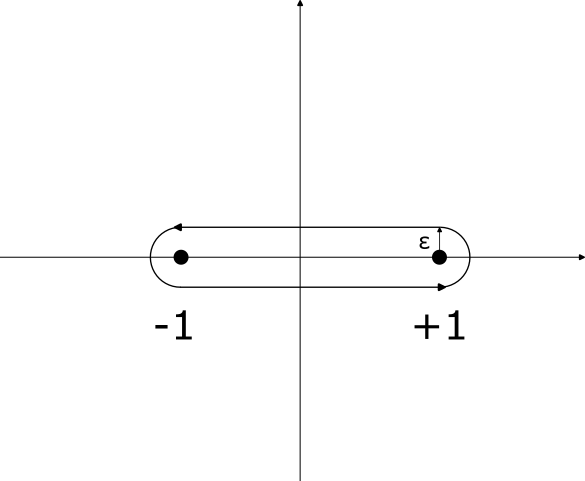
\includegraphics[scale=0.5]{images/racine_carree.png}
    \caption{Contour d'intégration pour la racine carrée.}
    \label{fig:racine_carree}
\end{figure}
En utilisant le résidu à l'infini, on obtient:
\[
\int_{\gamma} = - i 2 \pi \text{Res}_\infty f.
\]
Or:
\[
z\frac{-1}{z^2} \frac{1}{\sqrt{1-z^-2}} = -\frac{1}{\sqrt{z^2-1}}.
\]
En prenant la limite pour $z \to 0$, on en déduit:
\[
\text{Res}_\infty f = -i 2 \pi (i) = 2 \pi.
\]
Finalement, en faisant tendre $\epsilon$ vers $0$, la majoration ML montre que les intégrales sur les arcs de cercle se comportent comme $\sqrt{\epsilon}$ et tendent vers $0$ lorsque $\epsilon$ tend vers $0$. Concernant les intégrales sur les bords horizontaux, on remarque tout d'abord que sur le bord situé dans le demi-plan $\Im(z) < 0$ et avec la détermination choisie pour la racine carrée:
\begin{equation}
    \lim_{y \ to 0^-} \sqrt{1-z^2} \to \sqrt{1-x^2}.
\end{equation}
L'application $z \mapsto 1/\sqrt{1-z^2}$ se prolonge analytiquement dans un voisinage ouvert du segment $]-1,1[.$
En changeant de détermination pour $\sqrt{1-z}$ et pour $\eta>0$ assez petit, en posant $z= 1 + \eta \exp{i \theta},\, \theta \in ]-a,a[, 0 < a < \pi/2$, on peut écrire $\sqrt{1-z} = \sqrt{\eta} e^{i \theta/2}$ qui est bien définie.
L'intégrale le long du contour de la figure \ref{fig:racine_bords} vaut  $0$, l'intégrale sur le bord horizontal inférieur converge donc, pour $\epsilon \to 0^+$, vers:
\[
 \int_{-1}^1 \frac{dx}{\sqrt{1-x^2}}
\]
\begin{figure}
    \centering
    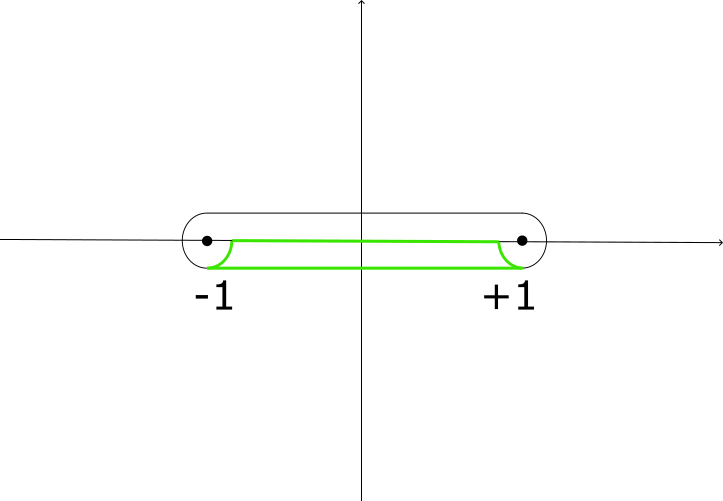
\includegraphics[scale=0.6]{images/contour_racine_bords.png}
    \caption{Bord inférieur de la coupure.}
    \label{fig:racine_bords}
\end{figure}
De même, l'intégral sur le bord supérieur converge vers:
\[
- \int_{-1}^1 \frac{dx}{\sqrt{1-x^2}}.
\] 
En regroupant les termes et en tenant compte de l'orientation, il vient:
\[
\int_{-1}^1 \frac{dx}{\sqrt{1-x^2}} = \pi.
\]
\begin{rem}
La technicité du calcul précédent ne milite pas en faveur de l'intégration dans le plan complexe. Ce n'est plus le cas, toutefois, si l'on s'intéresse à des intégrales de la forme:
\[
\int_0^x \frac{dt}{\sqrt{P(t)}}
\]
où $P$ est une application polynomiale de degré inférieur à $4.$
Toujours en utilisant les techniques présentées plus haut, on peut exprimer ces intégrales à partir des fonctions elliptiques de Jacobi, qui sont aisément calculables numériquement. On les rencontre en particulier lorsque l'on veut déterminer la distance géodésique entre deux points sur un ellipsoïde de révolution.
\end{rem}
\subsection{Intégrales faisant intervenir le logarithme}
Tout comme la racine carrée, le logarithme n'est pas une application holomorphe dans $\C$, il faut introduire une coupure, généralement $\R^-$ ou $\R^+.$ Soit l'application:
\[
f \colon z \mapsto \frac{\ln{z}}{1+z^2}
\]
On choisira de couper le plan complexe par la demi-droite $\R^+$, la détermination étant telle que $\ln(x+iy)_{y \to 0^+, x > 0} \to \ln(x)$ et
$\ln(x+iy)_{y \to 0^-, x > 0} \to \ln(x)+i 2 \pi.$ Sur le contour d'intégration $\gamma$ de la figure \ref{fig:contour_log}, le théorème des résidus donne, pour $R> 1, \epsilon < 1$:
\[
\int_\gamma f(z)dz = i2 \pi \left(
\text{Res}_i f + \text{Res}_{-i} f
\right)
\]
Les deux points singuliers étant des pôles simples, on a directement:
\[
\int_\gamma f(z)dz = i2 \pi \left(
\frac{\ln i}{2 i} + \frac{\ln (-i)}{- 2 i} \right)= (i 2 \pi)\left(- \frac{\pi}{2}\right).
\]
La majoration ML montre que les intégrales sur les deux arcs de cercle tendent vers $0$ pour $R \to +\infty, \epsilon \to O^+$, on en déduit:
\[
\int_{0}^{+\infty}\frac{\ln x}{1+x^2}dx - \int_{0}^{+\infty}\frac{i 2 \pi + \ln x}{1+x^2}dx = - i2 \pi \int_{0}^{+\infty}\frac{dx}{1+x^2}
\]
Soit:
\[
\int_{0}^{+\infty}\frac{dx}{1+x^2} = \frac{\pi}{2}
\]
Par le même procédé, on peut calculer les intégrales:
\[
\int_0^{+\infty} \frac{dx}{1 + x^n}=\frac{\pi}{n\sin{\pi/n}}
\]
En considérant:
\[
g\colon z \mapsto \frac{\ln^2 z}{1+z^n}dz
\]
on obtient également:
\[
\int_0^{+\infty} \frac{\ln x}{1 + x^n} dx = -\frac{\pi^2}{n^2}\frac{\cos{\pi/n}}{\sin^2{\pi/n}}.
\]

Le logarithme est souvent utilisé comme auxiliaire de calcul pour des intégrales sur $\R^+$ ou $\R^-$ ; c'est une technique à connaître.
\begin{figure}
    \centering
    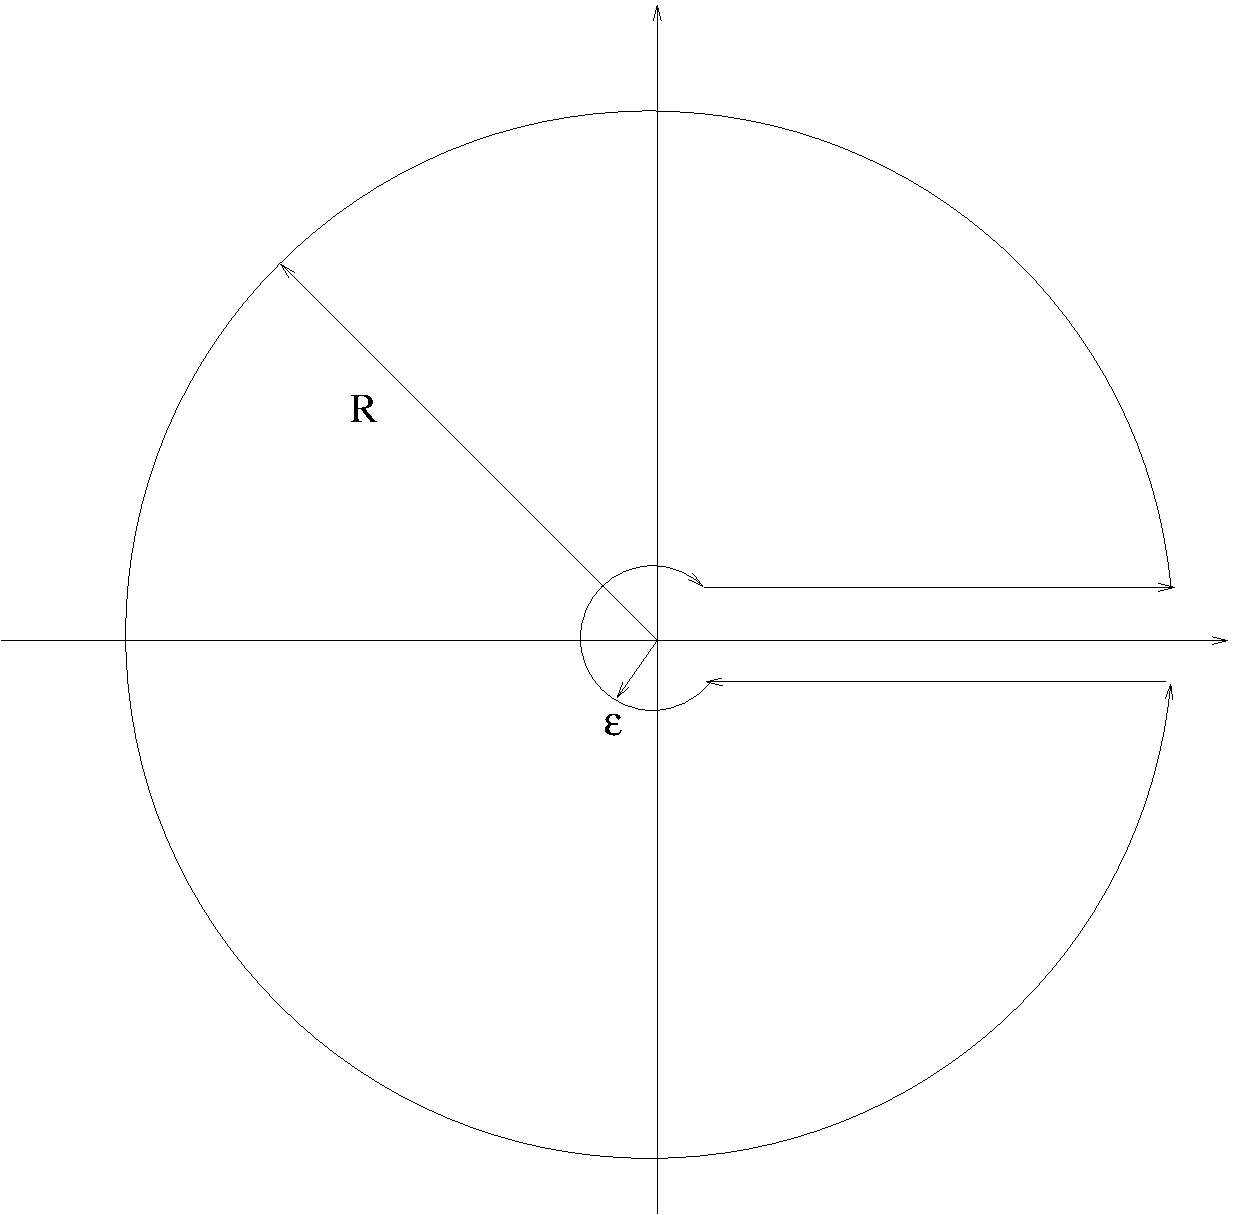
\includegraphics[scale=0.5]{images/contour_log.pdf}
    \caption{Contour d'intégration pour le logarithme complexe.}
    \label{fig:contour_log}
\end{figure}





\section{Exercices complémentaires}

\begin{exer}
Le résidu logarithmique d'une fonction $f(z)$ holomorphe est le résidu de la fonction $f^\prime(z)/f(z)$, dérivée de la fonction $\log f(z)$. 
\begin{MYenumerate}
\item Supposons que $a$ soit un zéro d'ordre $N$ de $f(z)$. Obtenir les premiers termes du développement en série de Laurent de la fonction $f^\prime(z)/f(z)$ et en déduire que $a$ est un pôle du premier ordre de résidu $N$.  
\item Soit $a$ un pôle d'ordre $N$ de $f(z)$. Considérer la fonction $g(z)=-1/f(z)$ et comparer $g^\prime(z)/g(z)$ à $f^\prime(z)/f(z)$. En déduire que $a$ est un pôle du premier ordre de $f^\prime(z)/f(z)$, de résidu $-N$.
\end{MYenumerate}
On a ainsi prouvé qu'aux zéros et aux pôles de $f(z)$, la dérivée logarithmique $f^\prime(z)/f(z)$ possède des pôles du premier ordre. De plus, en un zéro, le résidu logarithmique est égal à l'ordre du zéro, en un pôle à l'ordre du pôle précédé du signe moins.
\end{exer}

\begin{exer}
Soit $f$ une fonction holomorphe dans un domaine borné $\Omega$, sauf en un nombre fini de pôles $b_1,\cdots, b_m$ respectivement d'ordre $p_1, p_2, \cdots, p_m$, continue et ne s'annulant pas sur la frontière de ce domaine. La fonction $f$ a un nombre fini de zéros dans $\Omega$. Désignant par $a_1, a_2, \cdots, a_l$ les zéros respectifs de $f$ d'ordre respectifs $n_1,n_2,\cdots, n_l$.      
\begin{MYenumerate}
\item Appliquer le théorème des résidus à la dérivée logarithmique $f^\prime(z)/f(z)$.
\item En déduire la valeur de $N-P$, où $N$ et $P$ désignent respectivement le nombre de zéros et de pôles de $f$. En outre, chaque zéro et chaque pôle est compté autant de fois que son ordre l'indique.
\end{MYenumerate}
Notons que l'intégrale de la dérivée du logarithme (pour la détermination principale) s'écrit
\[\frac{1}{2 \pi i} \int_\gamma \diff \log f(z)  = \frac{1}{2 \pi i} \int_\gamma \diff \log \lvert f(z)\rvert +\frac{1}{2 \pi i} \int_\gamma \diff \text{arg} f(z).\]
La première intégrale de droite s'annule, tandis que la seconde est la variation totale $\Delta_\gamma \text{arg}f(z)$ de l'argument de $f(z)$, lorsque l'on décrit $\gamma$ divisé par $2 \pi$. Ainsi,
\[N-P=\frac{1}{2 \pi }\Delta_\gamma \text{arg}f(z).\]
\end{exer}

\begin{exer}
Soit $f(z)$ et $g(z)$ deux fonctions holomorphes à l'intérieur d'un contour $C$ donné et continue sur $C$.
\begin{MYenumerate}
\item Montrer que la dérivée logarithmique de $f(z)+g(z)$ est égale à la somme de la dérivée logarithmique de $f(z)$ et de $1+ g(z)/f(z)$.
\item Supposons que $\lvert f(z) \rvert > \lvert g(z) \rvert$ pour tout $z \in C$. En déduire que $\lvert f(z) \rvert > 0$ et $\lvert f(z) + g(z)\rvert >0$ sur $C$.
\item Lorsque $z$ décrit le contour $C$, le point $\omega=1+ g(z)/f(z)$ reste tout le temps dans le cercle $\lvert \omega -1 \rvert <1$. En déduire que le point $\omega$ ne peut faire le tour du point $0$, et donc que 
\[\Delta_C \text{arg}\left\{1 + \frac{g(z)}{f(z)}\right\}=0.\]
\item Conclure que les fonctions $f(z)+g(z)$ et $g(z)$ ont le même nombre de zéros à l'intérieur de $C$ (c'est le théorème de Rouché).
\end{MYenumerate}
\end{exer}


\begin{exer} On souhaite résoudre l'équation $e^z=1+2 z$ dans le disque unité. Une solution évidente est $z=0$, cherchons si il en existe d'autres. Pour cela appliquer le théorème de Rouché avec $f(z)=-2 z$ et $g(z)=e^z-1$.
\end{exer}


\begin{exer}
Le théorème des résidus peut servir à calculer des séries. Par exemple, pour calculer la somme de la série
\[\sum_{n=1}^\infty \frac{x}{n^2 \pi^2-x^2},\]
nous allons étudier l'intégrale 
\[I=\frac{1}{2 \pi i}\int_{C_n} \frac{\cot(w)}{w(w - z)} \diff w,\]
où le contour $C_n$ est le carré de sommets les quatre points $(\pm 1 \pm i)\cdot(n+\frac{1}{2})\cdot\pi$, et $z$ à l'intérieur du contour (donc $n$ assez grand).
\begin{MYenumerate}
\item Déterminer les pôles de la fonction en $w$ intégrée et en calculer les résidus (attention au pôle en zéro).
\item Utiliser le théorème des résidus pour calculer cette intégrale.
\item Majorer le module de $I$ pour $n \gg \lvert z \rvert$, et en déduire que $\lvert I \rvert \to 0$ lorsque $n \to \infty$.
\item En conclure que
\[\sum_{n=1}^\infty \frac{z}{n^2 \pi^2-z^2} = -\frac{1}{2}\cot z + \frac{1}{2 z}.\]
\end{MYenumerate}
\end{exer}

\newpage 
\subsection*{Un peu d'histoire \dots}

\begin{minipage}{0.2\linewidth}
\begin{center}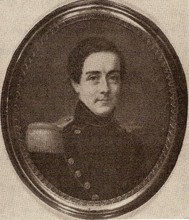
\includegraphics[width=2cm]{images/Laurent.jpg}\end{center}
\end{minipage}
\begin{minipage}{0.80 \linewidth}
\small{\paragraph*{Pierre Alphonse Laurent :} né le 18 juillet 1813 à Paris et mort le 2 septembre 1854 à Paris. Polytechnicien à 19 ans, il commence une carrière militaire et participe aux expéditions de Mascara et de Tlemcen. A son retour, il fut chargé de travaux visant à l'agrandissement du port de Havre. Il exerçait son activité scientifique sur son temps libre. Il contribua en physique à la théorie des ondes et introduisit en analyse complexe le développement en série qui porte son nom.}
\end{minipage}

\vspace*{2cm}


\begin{minipage}{0.2\linewidth}
\begin{center}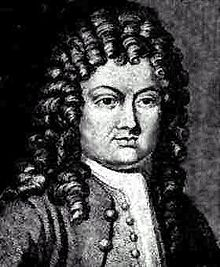
\includegraphics[width=2cm]{images/Taylor.jpg}\end{center}
\end{minipage}
\begin{minipage}{0.80 \linewidth}
\small{\paragraph*{Brook Taylor :} né à Edmonton (Borough d'Enfield, Londres, Angleterre) le 18 août 1685, et mort à Londres le 29 décembre 1731. Il invente l'intégration par parties et introduit le développement en série des applications différentiables. Il publie en 1715 deux ouvrages fondamentaux : \textit{Methodus incrementorum directa et inversa} dans lequel il aborde le problème des cordes vibrantes ainsi que le calcul des différences finies, et \textit{Linear Perspective}. Cependant, le terme de \textit{série de Taylor} n'apparaîtra qu'en 1786.}
\end{minipage}